\section{测试结果}

由于功能比较多,这里指展示几个比较关键的界面和测试情况。功能测试在编写程序时已有少量工作,暂时没有时间和能力做大量的测试。

程序使用简单的数字选择菜单,要求用户输入的时候会显示美元符号 \$ 当做命令提示符。

\subsection{教师模块}

\begin{figure}[htp]
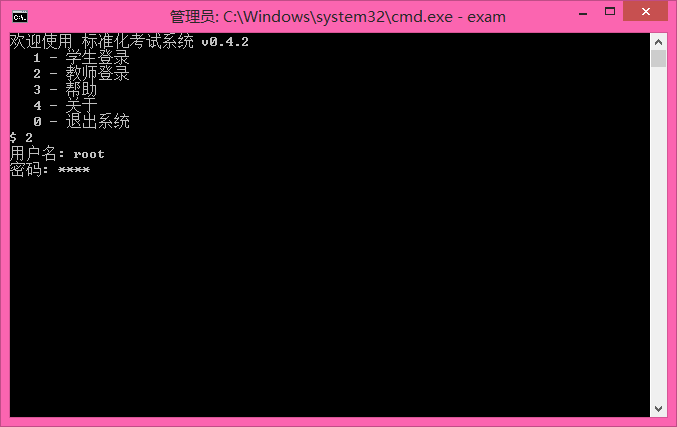
\includegraphics[width=\textwidth]{image/login_teacher.png}
\caption{\label{login_teacher}教师登录}
\end{figure}

如图~\ref{login_teacher}~,默认教师用户为 root ,密码 root,输入之后即可进入教师界面。

\subsubsection{题目增删改}

\begin{figure}[htp]
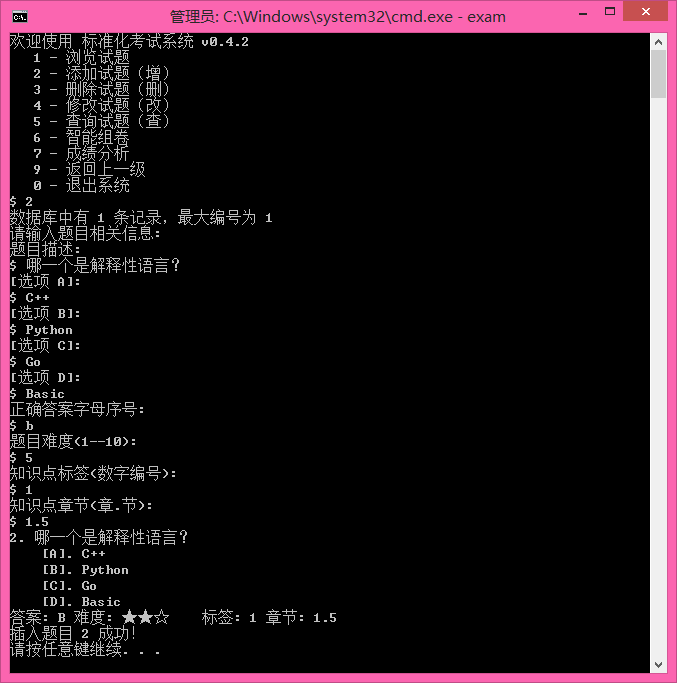
\includegraphics[width=\textwidth]{image/teacher_insert.png}
\caption{\label{teacher_insert}插入题目}
\end{figure}

进入教师界面,如图~\ref{teacher_insert}~,选择“添加试题(增)”,可以添加题目。输入题目信息时已经处理了大部分异常输入情况,在输入数字的地方必须输入数字,输入选项字母只需输入 A~D (大小写均可),输入字符串中可以输入空格。

\begin{figure}[htp]
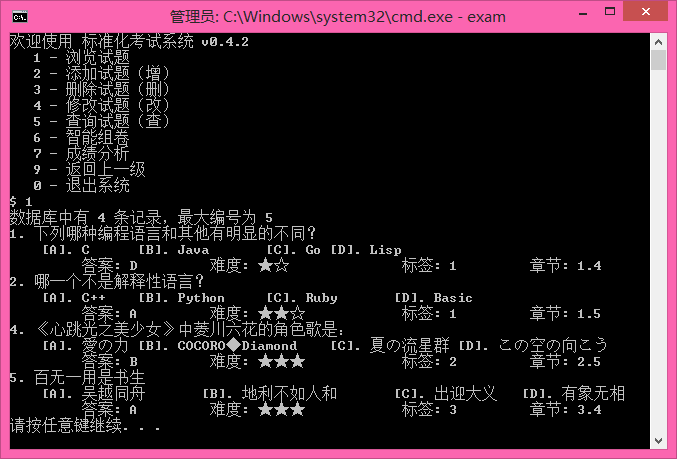
\includegraphics[width=\textwidth]{image/teacher_view.png}
\caption{\label{teacher_view}查看题目}
\end{figure}

如图~\ref{teacher_view}~,选择“浏览试题”,可以显示简短的题目信息列表。

\begin{figure}[htp]
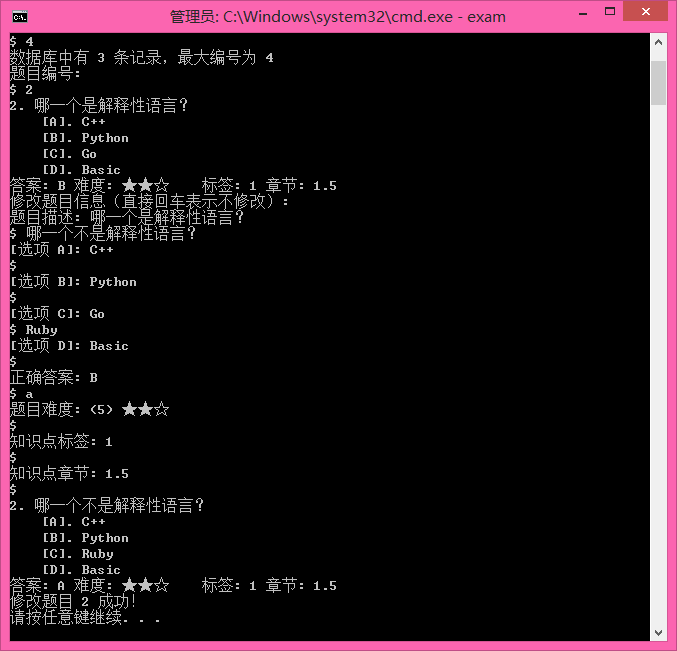
\includegraphics[width=\textwidth]{image/teacher_update.png}
\caption{\label{teacher_update}修改题目}
\end{figure}

如图~\ref{teacher_update}~,选择“修改试题(改)”后输入题号,可以修改已有题目。对于不想修改的信息可以按回车直接跳过,需要修改的若有输入也会有容错处理。

\begin{figure}[htp]
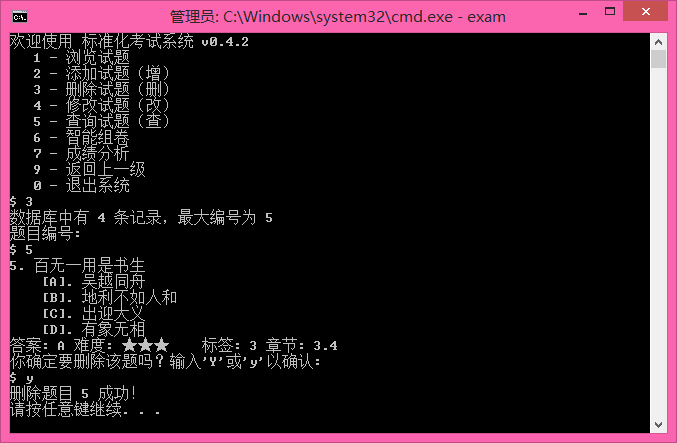
\includegraphics[width=\textwidth]{image/teacher_delete.png}
\caption{\label{teacher_delete}删除题目}
\end{figure}

如图~\ref{teacher_delete}~,选择“删除试题(删)”后输入题号,可以删除题库中的题目。由于删除操作的危险性,提示确认再删除。

\subsubsection{题目查询}

\begin{figure}[htp]
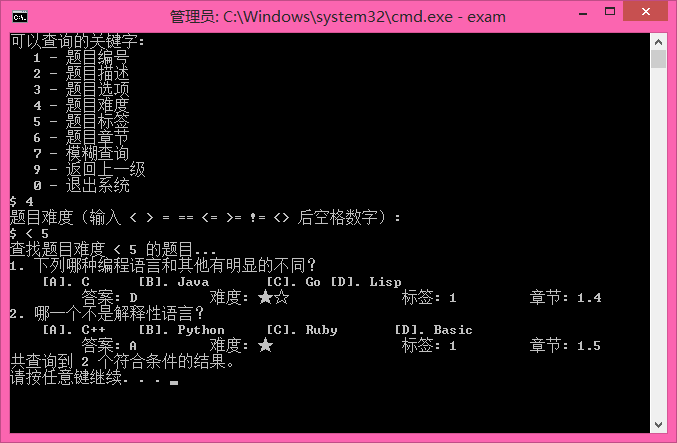
\includegraphics[width=\textwidth]{image/select_dif.png}
\caption{\label{select_dif}按难度查询}
\end{figure}

如图~\ref{select_dif}~,选择“题目难度”,可以按难度查询试题。你可以输入不等号后跟数字,比如这里输入了 \verb+< 5+ ,就能显示出所有难度小于5的题目。不等号可以是 \verb+< <= > >= = == != <>+,如果输错,默认为等于。

\begin{figure}[htp]
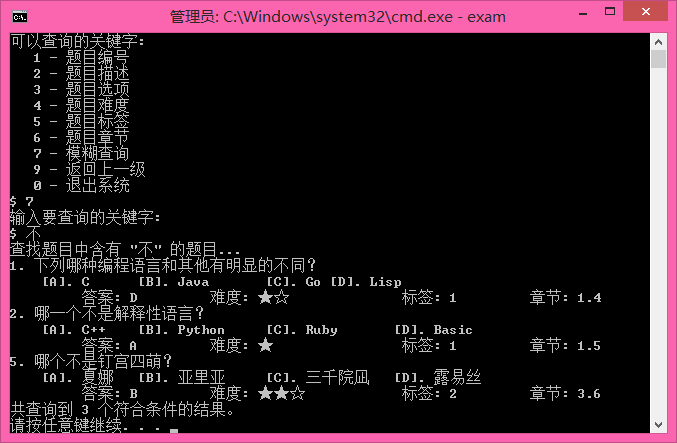
\includegraphics[width=\textwidth]{image/select_mul.png}
\caption{\label{select_mul}模糊查询}
\end{figure}

如图~\ref{select_mul}~,选择“模糊查询”,允许以一个关键字来查询所有题目属性。

\subsubsection{生成试卷}

\begin{figure}[htp]
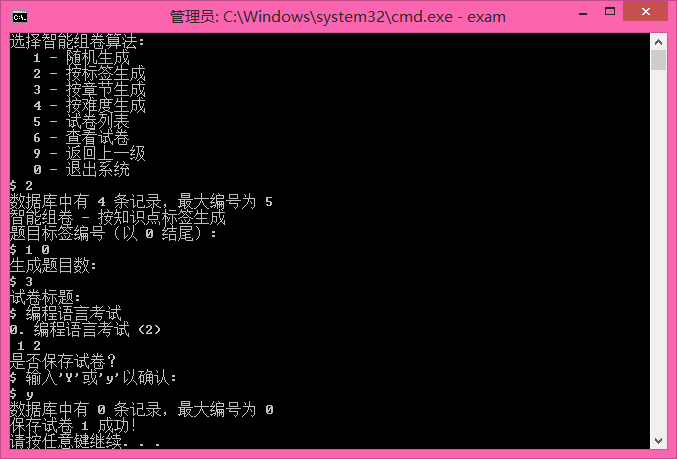
\includegraphics[width=\textwidth]{image/papar_random.png}
\caption{\label{papar_random}随机生成试卷}
\end{figure}

如图~\ref{papar_random}~,选择“随机生成”,输入题目数量和试卷标题,可以生成试卷。

\subsection{学生模块}

\begin{figure}[htp]
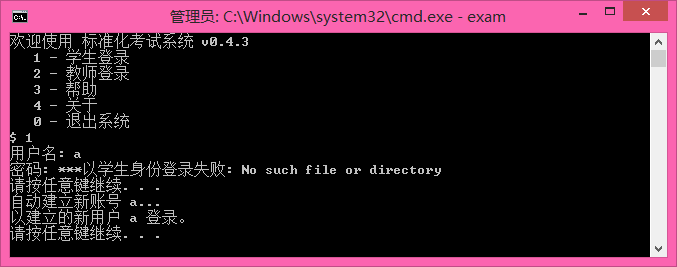
\includegraphics[width=\textwidth]{image/login_student.png}
\caption{\label{login_student}学生登录}
\end{figure}

如图~\ref{login_student}~,在主界面选择“学生登录”,任意输入用户名和密码,系统会自动建立学生用户并登录学生界面。

\begin{figure}[htp]
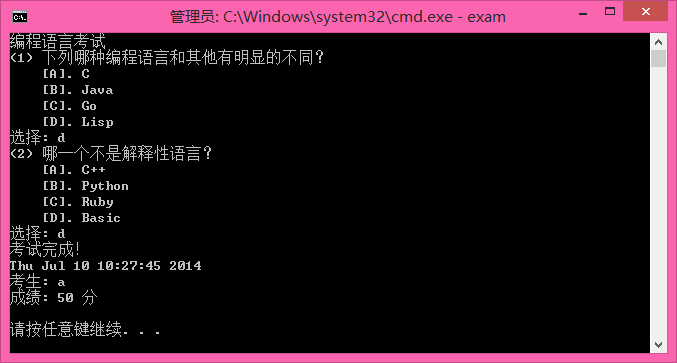
\includegraphics[width=\textwidth]{image/student_test.png}
\caption{\label{student_test}学生参与考试}
\end{figure}

如图~\ref{student_test}~,进入“做卷子”后,选择试卷后进入考试界面。依次做完所有试题之后会显示成绩并保存成绩到数据库。

\begin{figure}[htp]
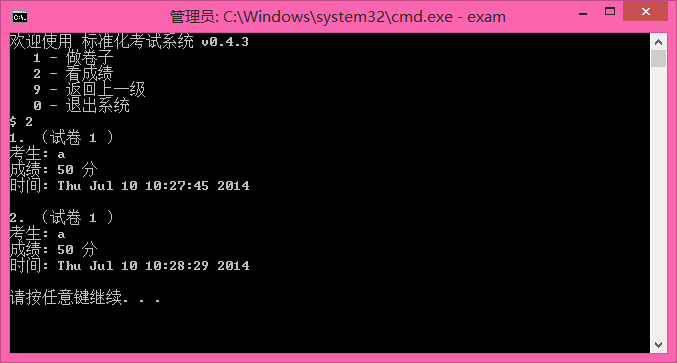
\includegraphics[width=\textwidth]{image/student_score.png}
\caption{\label{student_score}成绩列表}
\end{figure}

如图~\ref{student_score}~,学生可以查看自己的成绩列表。
